% !TeX root = ../main.tex
\section{Arquitectura del Sistema Propuesto}
\label{sec:arquitectura}

Para dotar al aprendizaje federado de trazabilidad y resistencia frente a comportamientos bizantinos, se propone una arquitectura híbrida desacoplada en tres planos operacionales: el plano de computación federada (Flower), el plano de almacenamiento direccionable fuera de cadena (IPFS) y el plano de consenso e inmutabilidad dentro de cadena (Hyperledger Besu). La Figura~\ref{fig:arq_sistema} ilustra la interacción integral entre estos componentes.

\begin{figure*}[t]
    \centering
    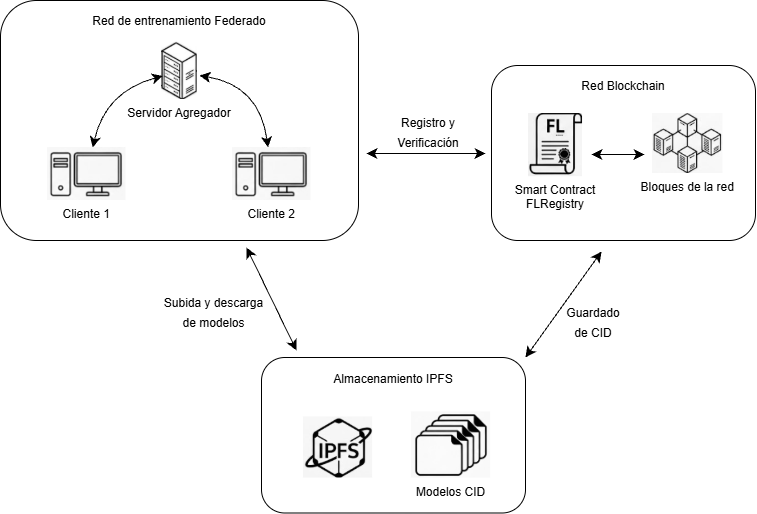
\includegraphics[width=0.88\textwidth]{figuras/ArqSistema.png}
    \caption{Arquitectura general del sistema híbrido: desacoplamiento entre el cómputo federado (Flower), el almacenamiento de pesos fuera de cadena (IPFS) y el registro inmutable de trazabilidad (Hyperledger Besu con IBFT 2.0).}
    \label{fig:arq_sistema}
\end{figure*}

\subsection{Diseño del Smart Contract: FLRegistry}
El componente de gobernanza y auditoría lógica se implementa mediante el contrato inteligente \texttt{FLRegistry}, codificado en Solidity (versión \texttt{0.8.10}). Su misión es registrar un historial criptográfico determinista de cada ronda sin albergar matrices numéricas masivas on-chain.
\\

\subsubsection{Estructuras de datos y persistencia}
La entidad nuclear del contrato es la estructura \texttt{ModelRound}, definida como:
\begin{verbatim}
struct ModelRound {
    uint256 roundNum;
    string modelHash;
    address author;
    uint256 timestamp;
}
\end{verbatim}
donde \texttt{roundNum} indexa la iteración federada, \texttt{modelHash} almacena el CID o digest SHA-256 del artefacto del modelo, \texttt{author} guarda la dirección pública Ethereum del emisor (\texttt{msg.sender}) y \texttt{timestamp} captura la marca temporal del bloque validado.
\\

El estado del contrato se organiza mediante dos tablas hash (\textit{mappings}) complementarias:
\begin{itemize}
    \item \texttt{mapping(uint256 => ModelRound) public \\ history}: almacena de forma secuencial los modelos globales agregados por el servidor al término de cada ronda $t$.
    \item \texttt{mapping(uint256 => mapping(address => \\ ModelRound)) public clientHistory}: indexa las contribuciones locales individuales de cada cliente en cada ronda, posibilitando la auditoría forense granular de las participaciones.
\end{itemize}

Adicionalmente, se mantienen los punteros de estado \texttt{latestRound} y el indicador booleano \texttt{hasModel} para optimizar lecturas directas $\mathcal{O}(1)$ sin requerir iteraciones sobre el almacenamiento persistente.
\\

\subsubsection{Primitivas de escritura y autenticación}
El contrato expone dos métodos transaccionales que alteran el estado y emiten el evento desacoplado \texttt{ModelUpdated}:
\begin{itemize}
    \item \texttt{updateModel(uint256 round, string memory hash)}: Invocado operacionalmente por el servidor tras converger el algoritmo de agregación. A nivel de diseño del banco de pruebas, la función se implementa con visibilidad pública para desacoplar el contrato de dependencias estáticas de despliegue; no obstante, la EVM registra de forma inmutable la dirección emisora en el campo \texttt{author} (\texttt{msg.sender}). Esto permite a los clientes verificar criptográficamente frente a la clave pública autorizada del servidor que el modelo global sellado proviene legítimamente del agregador del consorcio.
\end{itemize}

\subsubsection{Primitivas de lectura y verificación}
Para no sobrecargar la red con costes de ejecución, las consultas de verificación se implementan como funciones \texttt{view}, las cuales se resuelven localmente en el nodo RPC sin consumir gas:
\begin{itemize}
    \item \texttt{getLastModel()}: Permite a cualquier cliente recuperar el CID del último modelo global consolidado y su marca de tiempo.
    \item \texttt{getClientModel(uint256 round, address client)}: Permite al servidor y a auditores externos cotejar el CID reportado por un cliente frente a su registro on-chain firmado.
\end{itemize}

\subsection{Flujo Operacional y Doble Verificación Cruzada}
El ciclo de vida del entrenamiento federado se estructura en una fase de inicialización única seguida de un protocolo iterativo con verificación bidireccional estricta, como se resume a continuación:
\\

\subsubsection{Fase 0: Arranque y Modelo Base (Ronda 0)}
Antes de iniciar la concurrencia:
\begin{enumerate}
    \item Se inicializa la red Besu con consenso IBFT 2.0 y el daemon IPFS.
    \item Se despliega \texttt{FLRegistry} registrando su dirección y ABI en un descriptor JSON distribuido.
    \item El servidor instancia los pesos iniciales $w^{(0)}$, los serializa y los almacena en IPFS, recibiendo un CID inicial $\text{CID}_0$.
    \item El servidor ejecuta \texttt{updateModel(0, }$\text{CID}_0$\texttt{)}, fijando el punto de partida auditable para todos los participantes. \\
\end{enumerate}

\subsubsection{Fase 1: Verificación Descendente (Cliente protege frente a Servidor)}
Al recibir la señal de inicio de ronda junto con los pesos candidatos $w_{cand}^{(t)}$ vía gRPC (Figura~\ref{fig:flujo_cliente_verif}):
\begin{enumerate}
    \item El cliente consulta la Blockchain invocando \texttt{getLastModel()} y obtiene el $\text{CID}_{reg}^{(t-1)}$ oficial.
    \item El cliente descarga el modelo referenciado desde IPFS y realiza una verificación bit a bit tensor por tensor frente a $w_{cand}^{(t)}$.
    \item Si se detecta cualquier discrepancia entre los pesos entregados y el compromiso sellado en la cadena, el cliente \textbf{aborta el entrenamiento inmediatamente}, neutralizando ataques donde un servidor comprometido intente inyectar modelos sesgados selectivamente a clientes concretos.
\end{enumerate}

\begin{figure}[H]
    \centering
    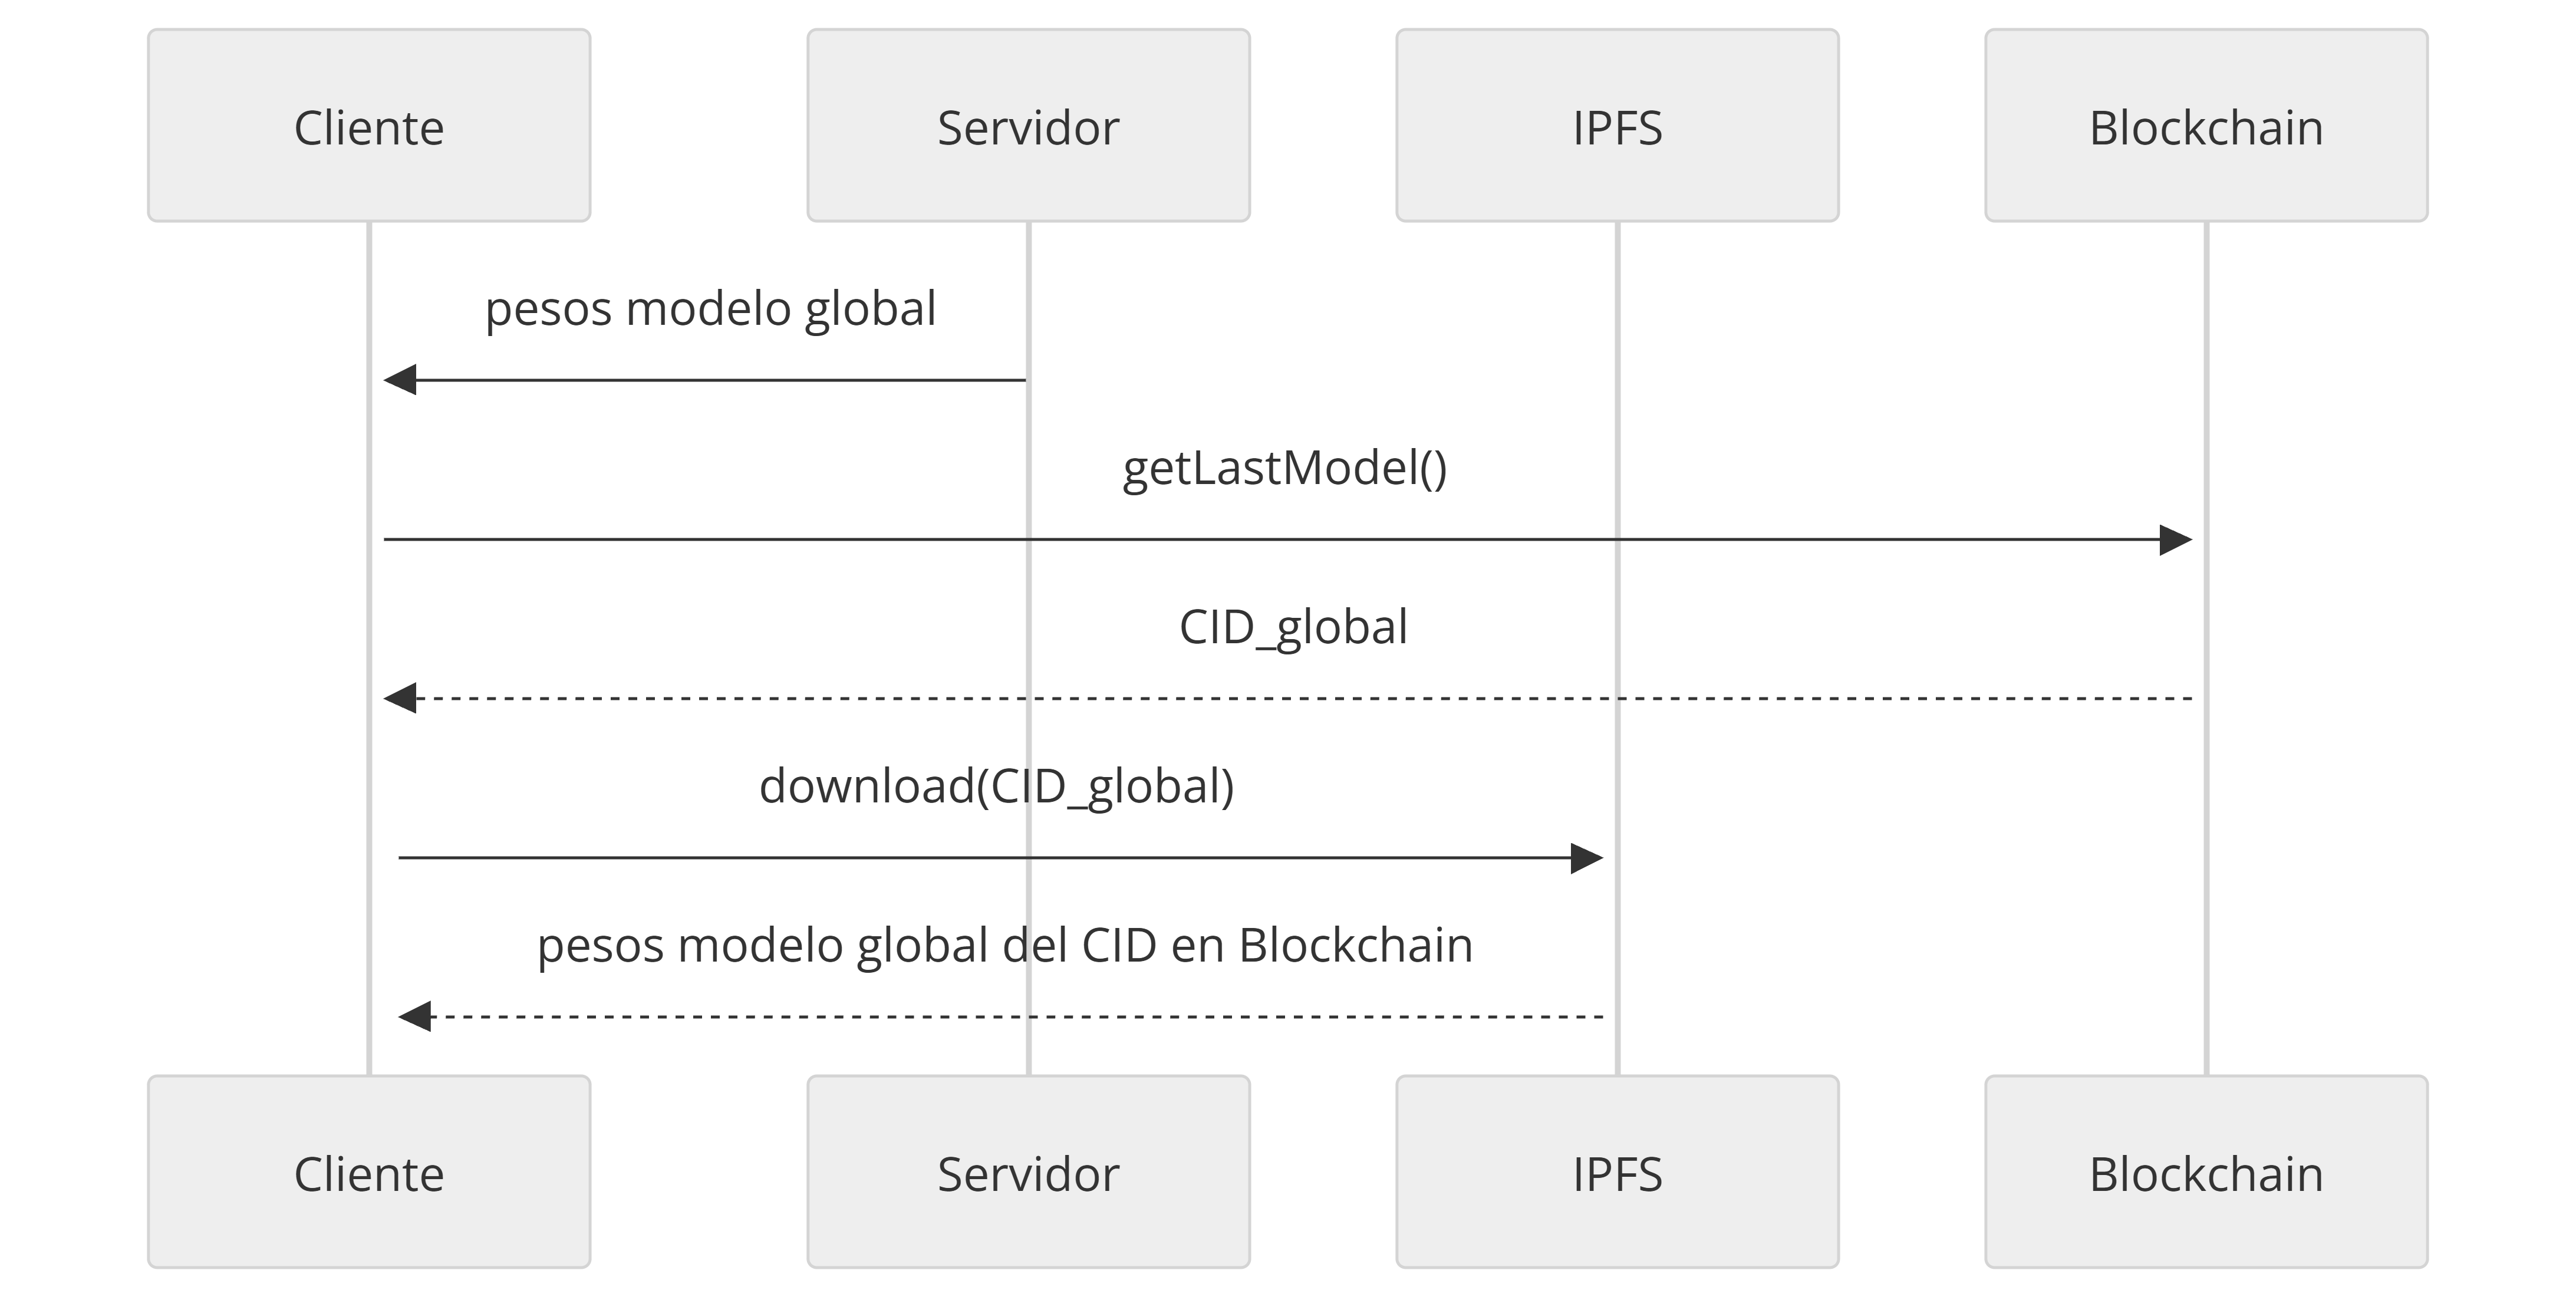
\includegraphics[width=\columnwidth]{figuras/inicio_ronda_good.png}
    \caption{Fase 1: Verificación descendente en el cliente: cotejo del modelo recibido frente al CID registrado on-chain y descargado de IPFS.}
    \label{fig:flujo_cliente_verif}
\end{figure}

\subsubsection{Fase 2: Entrenamiento Local y Registro de Contribución}
Si la comprobación previa es satisfactoria (Figura~\ref{fig:flujo_cliente_entreno}):
\begin{enumerate}
    \item El cliente ejecuta el entrenamiento local con su partición privada de datos.
    \item Serializa los nuevos pesos locales $w_k^{(t)}$ y los almacena en IPFS, obteniendo $\text{CID}_k^{(t)}$.
    \item Emite una transacción firmada con su clave privada invocando \texttt{registerClientModel(}$t$, $\text{CID}_k^{(t)}$\texttt{)} y aguarda el recibo (\textit{receipt}) de inclusión en el bloque IBFT 2.0.
    \item Retorna a Flower los parámetros junto con el identificador $\text{CID}_k^{(t)}$ y su clave pública.
\end{enumerate}

\begin{figure}[H]
    \centering
    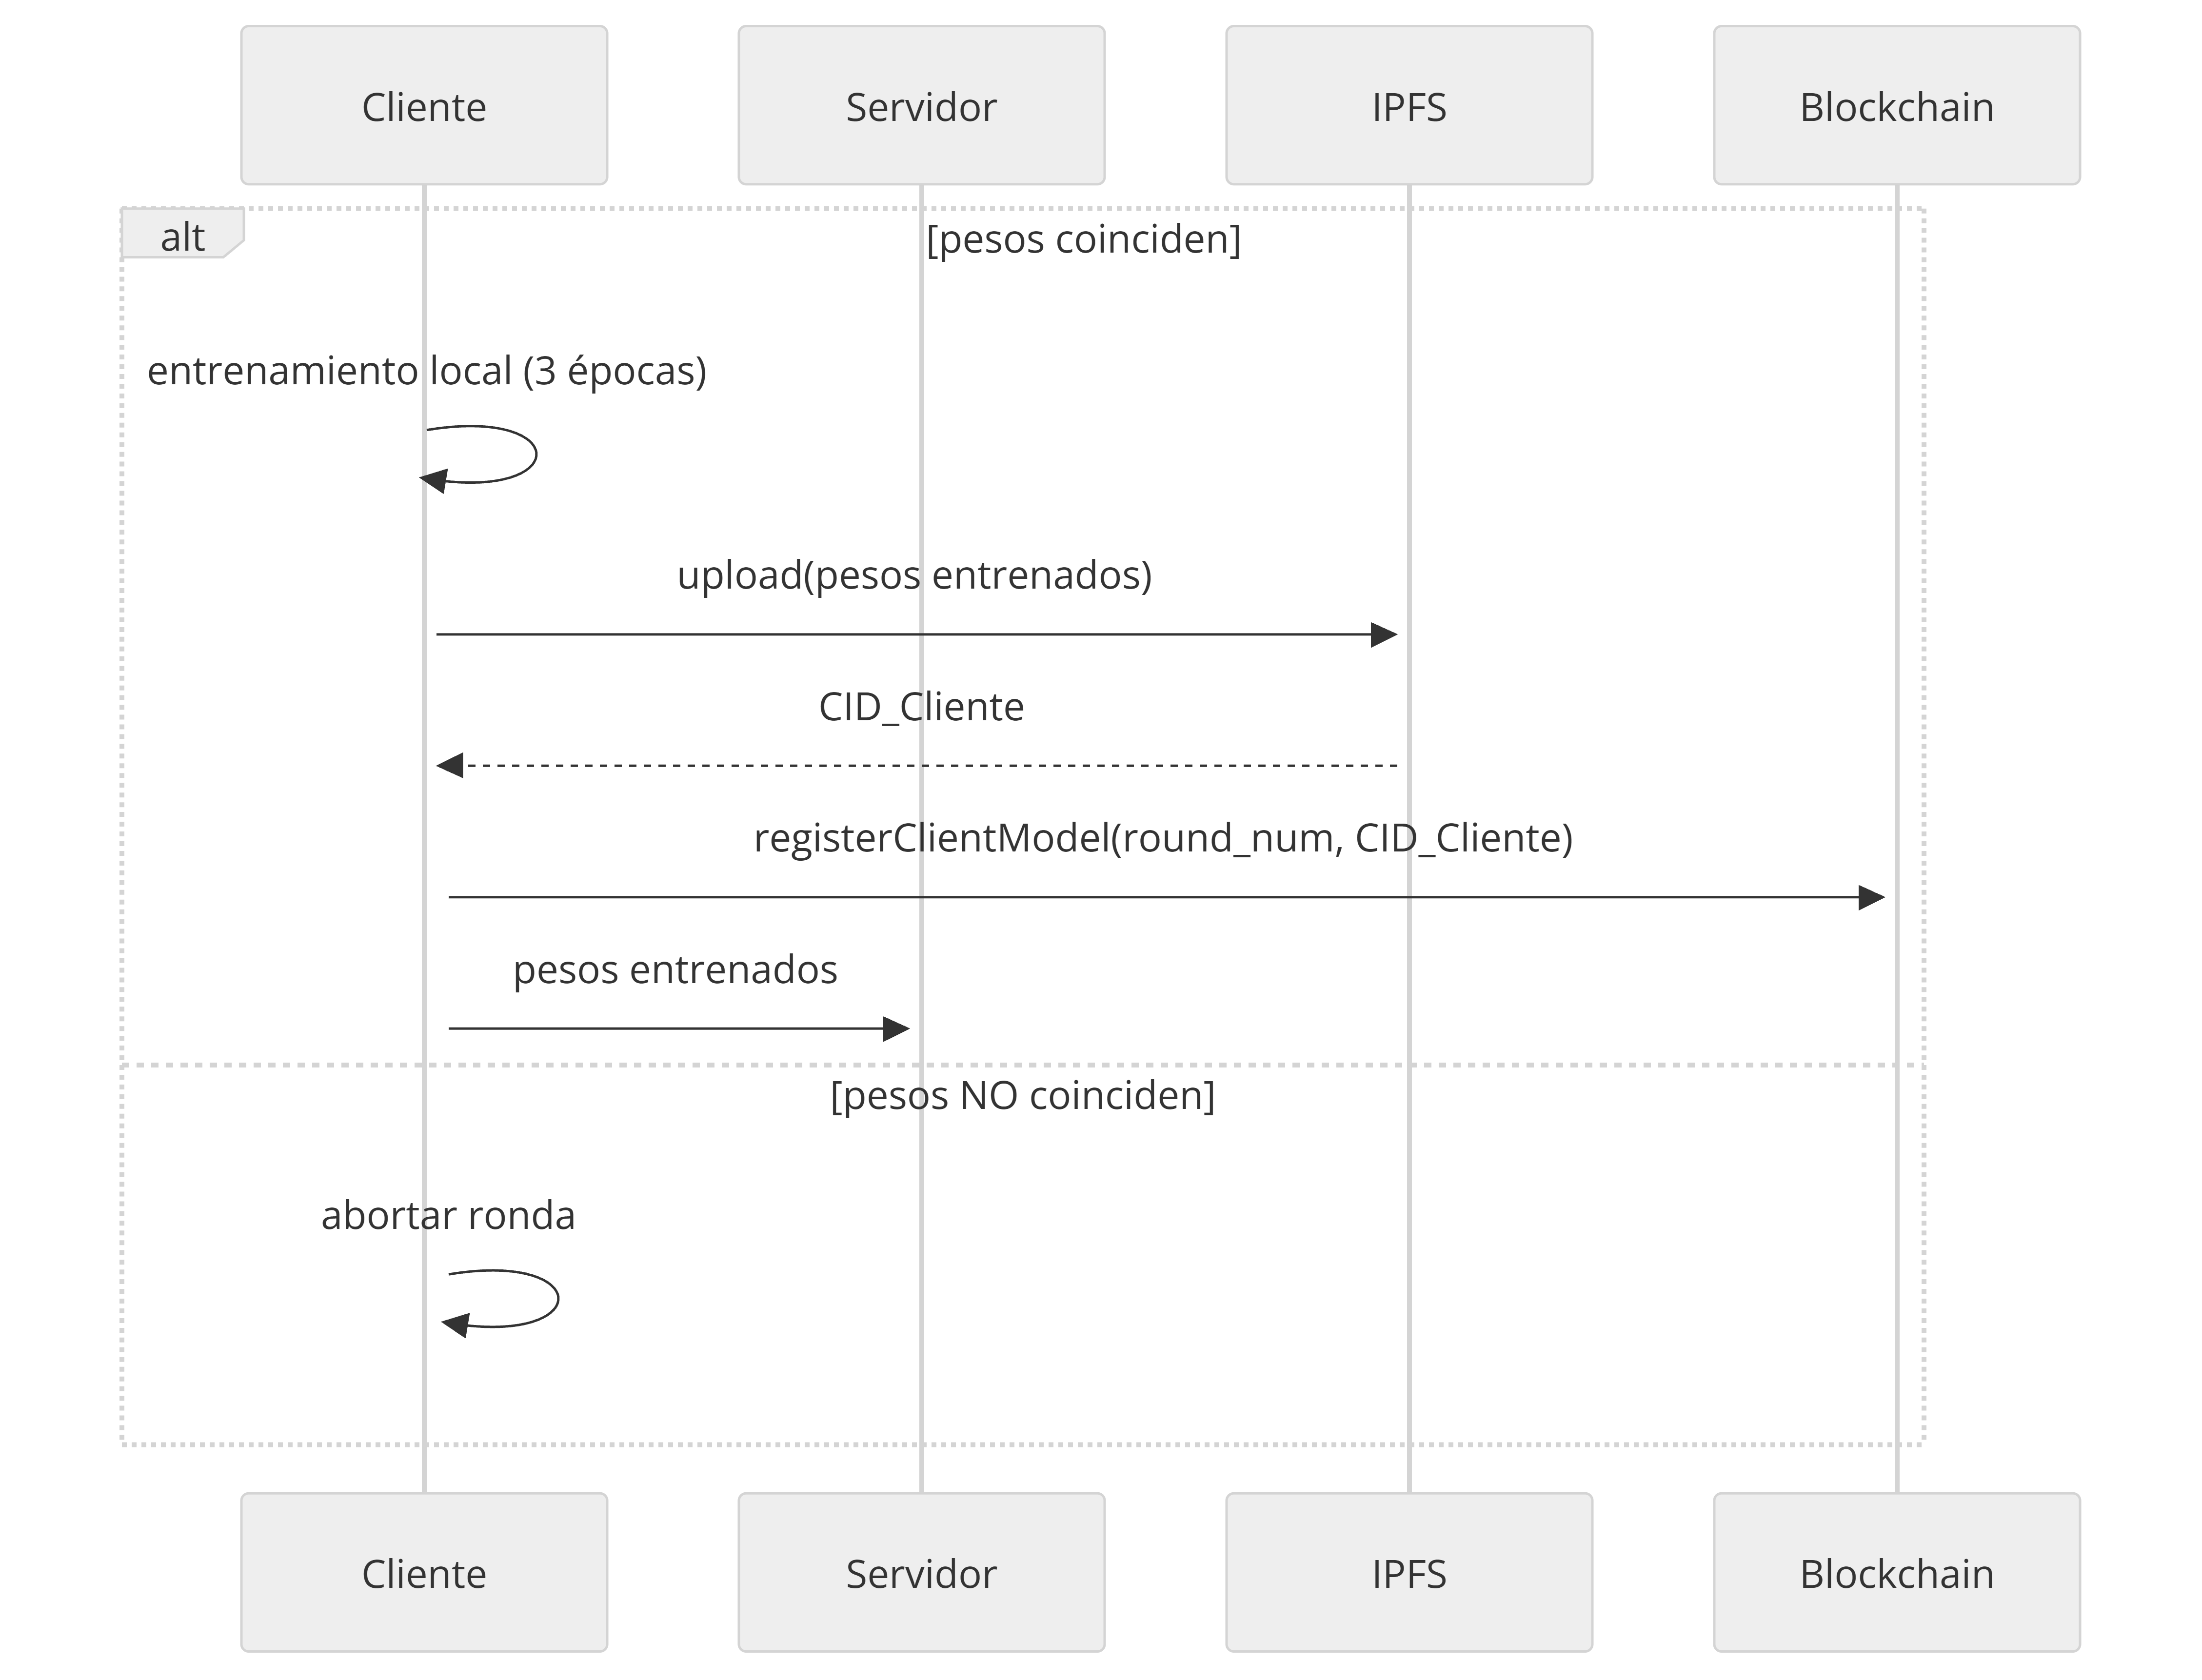
\includegraphics[width=\columnwidth]{figuras/entrenamiento.png}
    \caption{Fase 2: Entrenamiento local en el cliente, subida de pesos a IPFS y transacción firmada a Hyperledger Besu.}
    \label{fig:flujo_cliente_entreno}
\end{figure}

\subsubsection{Fase 3: Verificación Ascendente y Agregación Global}
Al recibir los pesos de los clientes en el servidor agregador (Figura~\ref{fig:flujo_servidor_agregacion}):
\begin{enumerate}
    \item Para cada cliente $k$, el servidor consulta \texttt{getClientModel(}$t$, $\text{address}_k$\texttt{)} en la Blockchain.
    \item Comprueba que el CID reportado por gRPC coincida con el hash inmutable registrado y firmado por el cliente. Si la comprobación falla, la contribución es descartada de forma preventiva.
    \item Aplica la agregación ponderada FedAvg únicamente sobre las contribuciones debidamente auditadas:
    \begin{equation}
    w^{(t+1)} = \sum_{k \in \mathcal{K}_{valid}} \frac{n_k}{n_{valid}} \, w_k^{(t)}
    \end{equation}
    \item Sube el nuevo modelo consolidado a IPFS, obteniendo $\text{CID}_{global}^{(t+1)}$, y lo sella en Besu invocando \texttt{updateModel(}$t+1$, $\text{CID}_{global}^{(t+1)}$\texttt{)}.
\end{enumerate}

\begin{figure}[H]
    \centering
    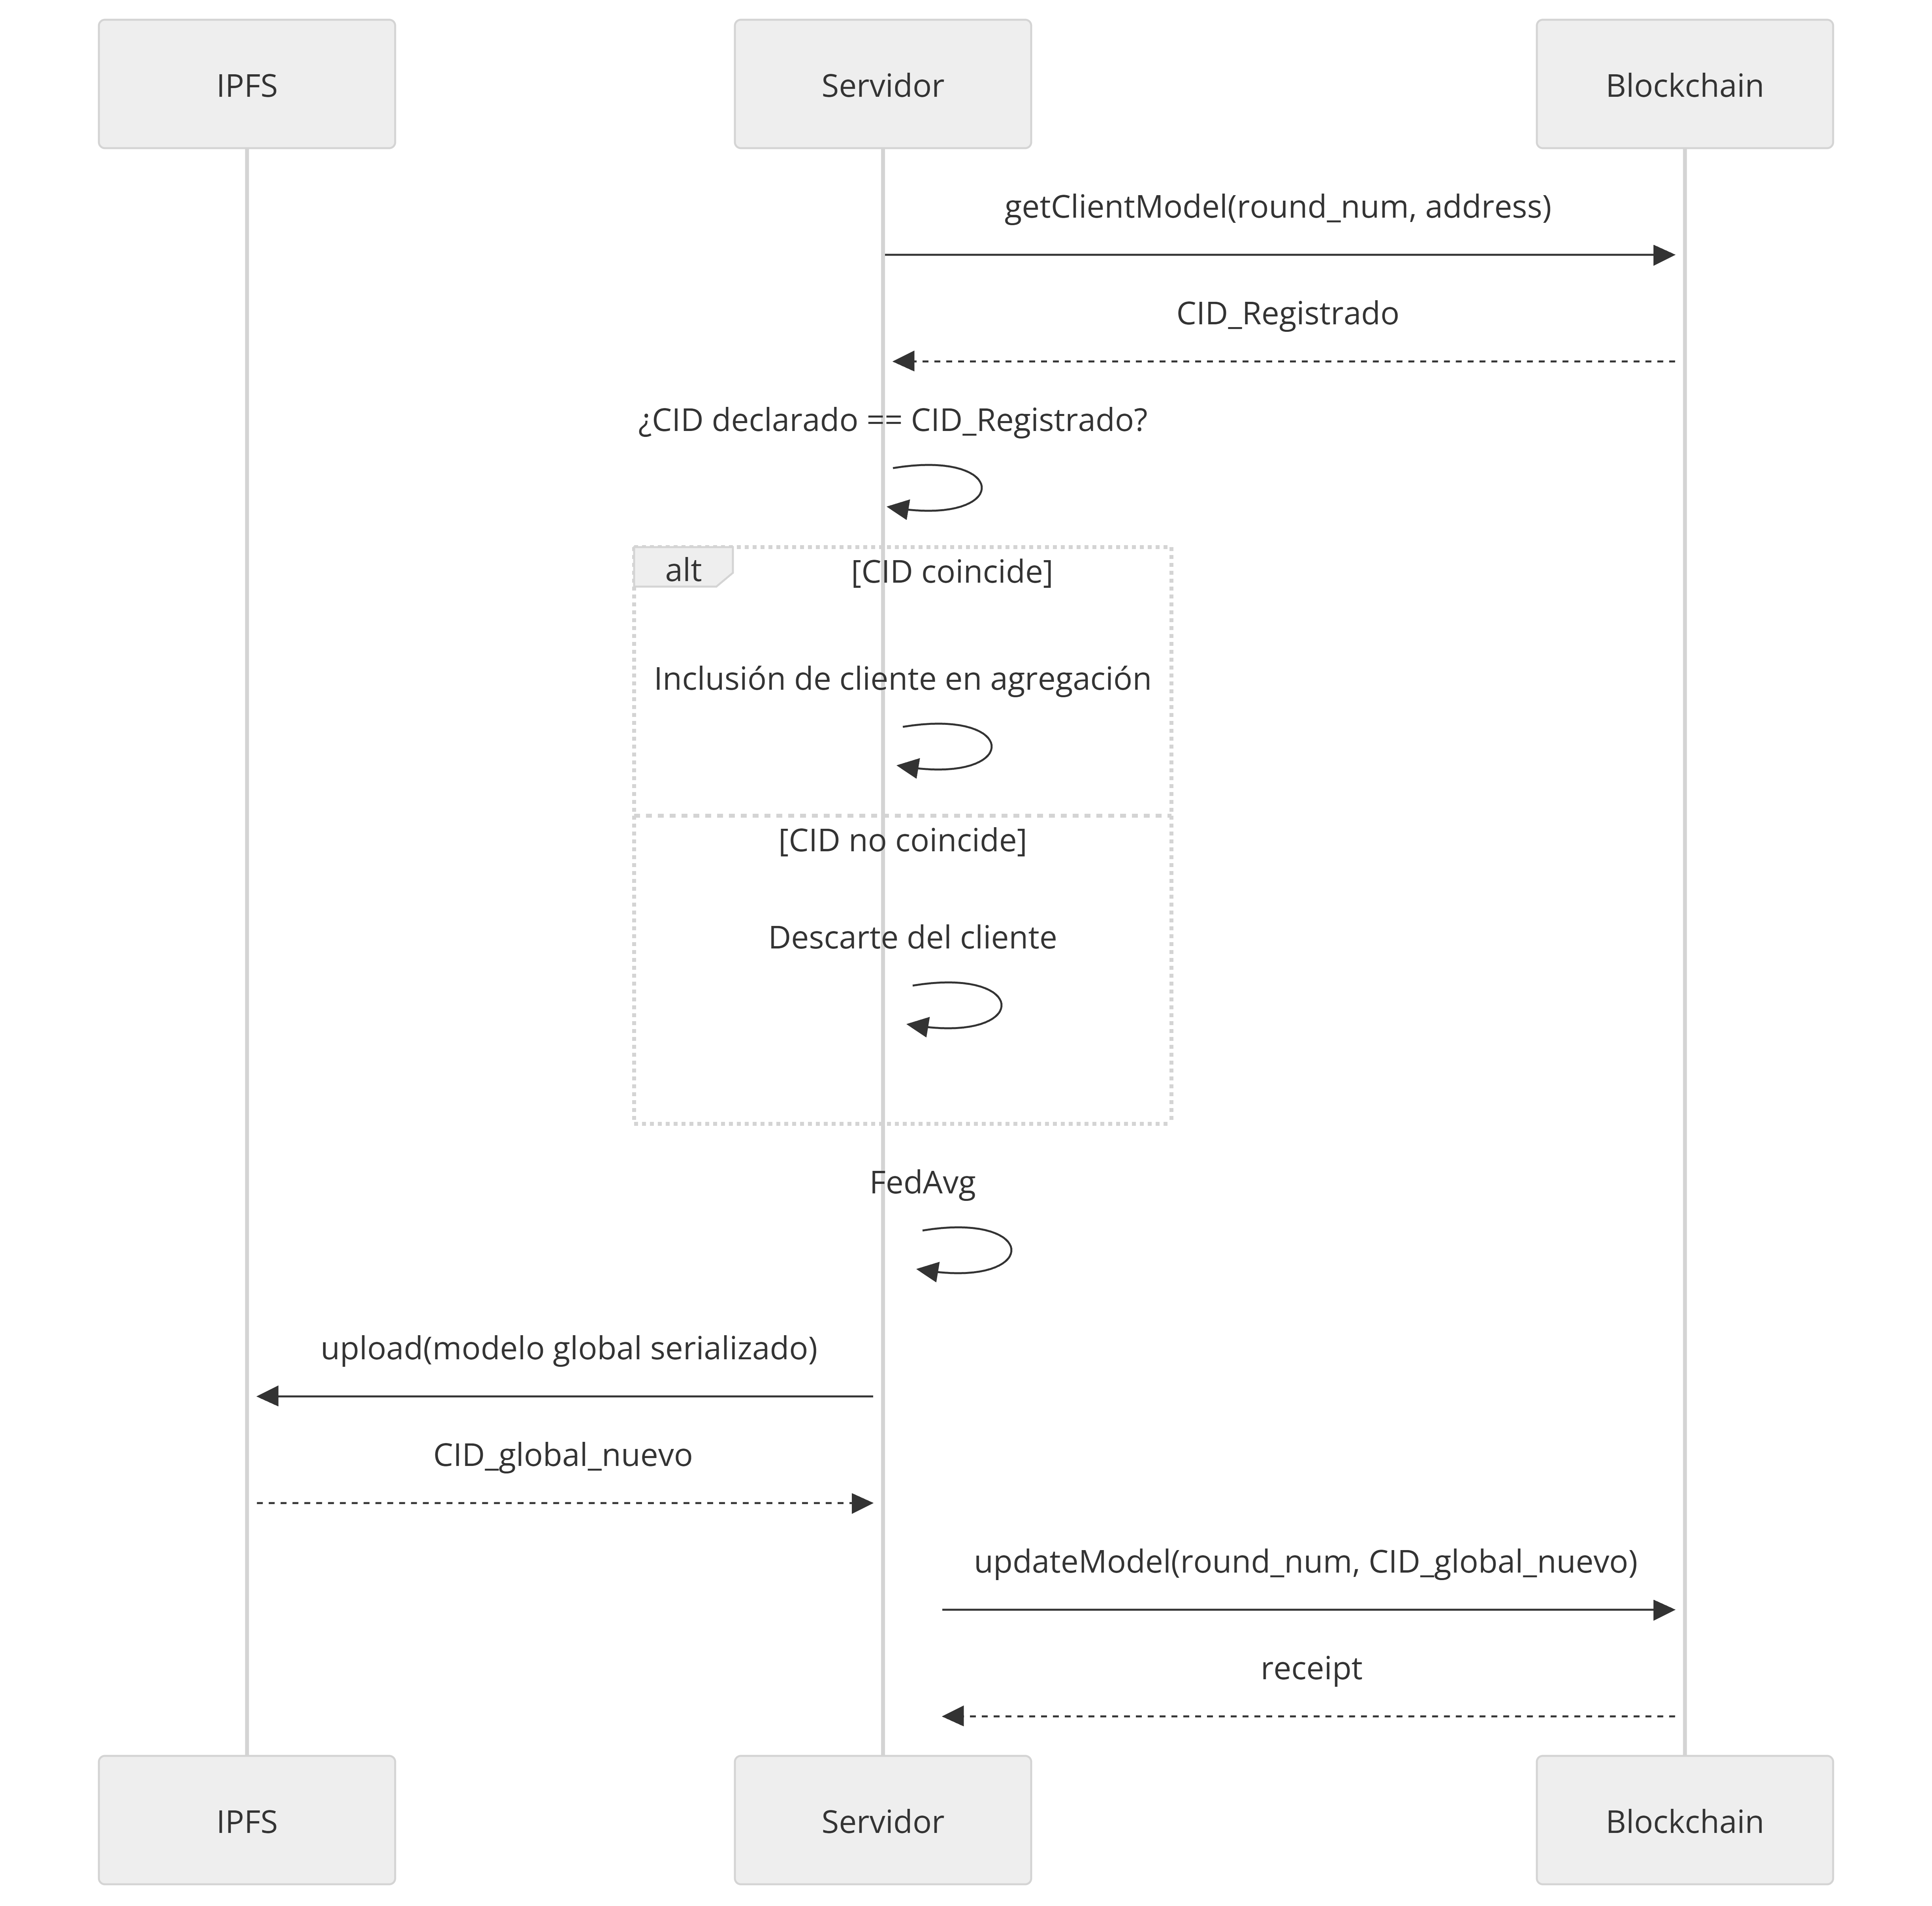
\includegraphics[width=\columnwidth]{figuras/fin_ronda.png}
    \caption{Fase 3: Verificación ascendente en el servidor: validación de CIDs on-chain, agregación FedAvg y sellado global de ronda.}
    \label{fig:flujo_servidor_agregacion}
\end{figure}

Este mecanismo garantiza trazabilidad completa de extremo a extremo, no repudio y aislamiento de participantes disidentes.
